\chapter{Einführung}
Die Variationsrechnung ist primär an kritischen Punkten/Minimierern von Funktionalen der Form:
\begin{equation}
    \mathcal{F}: \mathcal{A} \to \overline{\mathbb{R}}
\end{equation}
interessiert. Hierbei bezeichnet \(\mathcal{A}\) einen im Allgemeinen \(\infty-\)dimensionalen Unterraum eines normierten Raumes \(\mathcal{X}\).\\
Bevor wir uns dem eigentlichen Thema zuwenden, werden wir es sowohl mathematisch, als auch physikalisch motivieren. Der mathematischen Motivation dient eine kurze Wiederholung der klassischen direkten Methode. Wiederholung in dem Sinne, dass sie in dem Vortrag zuvor bereits vorgestellt wurde, jedoch von derart großer Bedeutung für das Thema Relaxierung ist, dass wir sie nochmals erwähnen. Im zweiten Teil motivieren wir den Nutzen dann durch ein physikalisches Anwendungsbeispiel.\\

\textbf{Bemerkung:} Insofern nicht explizit angegeben, ist mit Integration immer Integration bezüglich des Lebesgue-/Hausdorff-Maßes gemeint.\\
\section{Wiederholung: Die direkte Methode}
\textit{Quelle für Definitionen/Sätze dieses Kapitels: \cite{CalcVar}}\\[0.1cm]
Zunächst bedienen wir uns einem Lemma, das aus den Analysis-\\Grundlagenvorlesungen schon bekannt sein sollte:\\
\pgfsetfillopacity{0.2}\colorbox{lemyellow}{\begin{minipage}{16cm}{\textcolor{black}{\pgfsetfillopacity{1}}{\label{lem1.1}}}
\textbf{Lemma 1.1 (Cantor's intersection theorem):} Sei \((K_i)_{i \in I}\) eine Familie kompakter Mengen eines Hausdorffraums mit beliebiger Indexmenge \(I\). Dann gilt:
\begin{equation}
    (\bigcap_{i \in J} K_i \neq \emptyset \, \forall J \subset I) \Rightarrow (\bigcap_{i \in I} K_i \neq \emptyset)
\end{equation}
\end{minipage}}

\textsc{Beweis:} Das Lemma ist aus den Grundlagenvorlesungen bekannt und ist auch als duale Version der Überdeckungskompaktheit nicht sehr schwer zu beweisen.\QEDB\\
\\
Nun also die besagte direkte Methode in der allgemeinsten Version:\\
\pgfsetfillopacity{0.2}\colorbox{theored}{\begin{minipage}{16cm}{\textcolor{black}{\pgfsetfillopacity{1}}{\label{theo1.2}}}
\textbf{Satz 1.2 (Die direkte Methode, topologische Version):} Sei \(\mathcal{A}\) ein topologischer, nicht-leerer Hausdorff-Raum, sowie \(\mathcal{F}\) ein Funktional wie in (1.1). Gilt nun:
\begin{enumerate}
    \item Die Subniveaumengen \(\{w \in \mathcal{A}\, | \, \mathcal{F}[w] \le s,\, s \in \mathbb{R}\}\) sind relativ kompakt in \(\mathcal{A}\) und
    \item \(\mathcal{F}\) ist unterhalbstetig auf \(\mathcal{A}\),
\end{enumerate}
dann existiert ein Minimierer \(u \in \mathcal{A}\) von \(\mathcal{F}\).
\end{minipage}}

\textsc{Beweis:} Nach den Voraussetzungen sind die Subniveaumengen kompakt in \(\mathcal{A}\). Diese kann man nun als Schnitt über das Infimum (das \(< \infty\) angenommen werden kann, sonst ist jedes \(u \in \mathcal{A}\) ein Minimierer und die Aussage trivial) betrachten und mit [\ref{lem1.1}][Lemma 1.1] die Behauptung folgern.\QEDB\\

\section{Physikalische Motivation}
\textit{Quelle für Definitionen/Sätze dieses Kapitels: \cite{CalcVarBSchmidt}}\\[0.1cm]
Wir betrachten nun das bekannte Segler-Problem und zeigen dann anhand eines Spezialfalls (den man in Literatur/Internet auch unter Bolza-Problem finden kann), wie bei einem realen physikalischen Problem die direkte Methode fehlschlagen kann.\\
Betrachten wir also einen Segler auf einem Fluss \([a,b] \times [-1,1]\) auf \(\{(x,w(x))\, | \, x \in [a,b]\}\) mit Gegenwind \((-1,0)\). Nun wird der Segler am effektivsten segeln, indem er die Windkraft im optimalen Winkel \(\alpha > 0\) ausnutzt. Der Kurs muss also \(|w'(x)|=\alpha\) erfüllen. Wir sind hierbei also an folgendem variationellem Problem interessiert:
\begin{equation}
    \text{max} \leftarrow \mathcal{F}[w]:=\int_{a}^b F(w'(x)) \,dx 
\end{equation}
Diese Modellierung ist sehr idealistisch, da wir nicht die Strömung \(S(w(x))\) des Flusses berücksichtigen. Die bessere Modellierung lautet also:
\begin{equation}
    \text{max} \leftarrow \mathcal{F}[w]:=\int_{a}^b F(w'(x)) + S(w(x))\, dx
\end{equation}
Bildlich könnte man sich diese Situation folgendermaßen vorstellen:
\begin{figure}[!h]
    \centering
    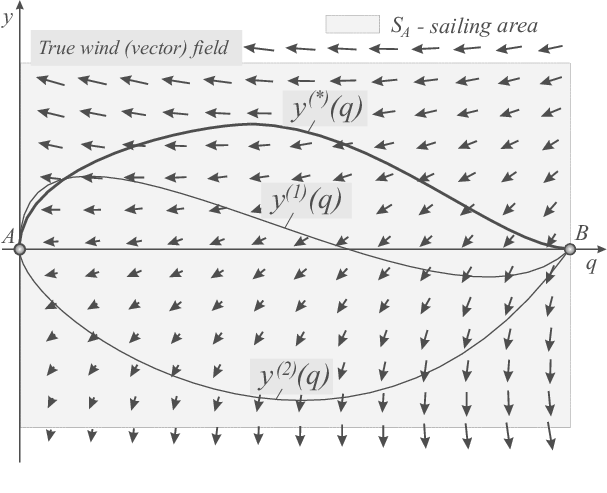
\includegraphics[scale=0.42]{figures/Sailboat-trajectory.png}
    \caption{Graphische Veranschaulichung des Seglerproblems\cite{Sailboat}}
    \label{fig:sail}
\end{figure}\\

Zu sehen sind Beispiele an zulässigen Trajektoren von Punkt A nach Punkt B mit \(y^*(q)\) der approximierten Optimalroute.\\
Wir haben dieses Problem gerade so modelliert, dass die Maxima von F und S \\gerade \(F_{\text{max}} = F(\pm \alpha)\) und \(S_{\text{max}} = S(0)\) sind. Wir sehen also ein, dass das Supremum gegeben ist durch \((F_{\text{max}} + S_{\text{max}})(b-a)\). Dies führt jedoch zu einem Problem, denn damit besitzt das Funktional \(\mathcal{F}\) keinen Maxmierer, da \(u = 0\) f.ü. gelten müsste, weshalb dann \(u' = 0 \neq \pm \alpha\) f.ü. wäre.\\
Doch woran ist die Existenztheorie hier genau gescheitert? Dazu wollen wir nun, wie bereits oben schon einmal erwähnt, den Bolza-Spezialfall (als duale Version des obigen Maximierungsproblems) mathematisch genauer unter die Lupe nehmen:\\
Sei \(a < b \in \mathbb{R}\) und
\begin{equation}
    \mathcal{F}:W^{1,4}(]a,b[) \to \mathbb{R}_0^+,\,\mathcal{F}[w] := \int_{a}^b ((w')^2 - 1)^2 + w^4\,dx
\end{equation}
Da \(W^{1,4}(]a,b[)\) ein Hilbertraum ist, ist er insbesondere ein reflexiver Banachraum. Damit gilt Bedingung (1) der direkten Methode, da \(\mathcal{F}\) Norm-koerziv ist (mit der Young-\\Ungleichung gilt \((w')^2 \le  \frac{(w')^4}{4} + 1\) und in reflexiven Banachräumen (auf einem schwach abgeschlossenem Unterraum; schwach im Sinne der schwachen Topologie (Initialtopologie zum Dual-Raum)) folgt Bedingung (1) der direkten Methode aus Norm-\\Koerzivität; für einen Beweis verweisen wir aus Zeitgründen auf \cite{CalcVar}[Seite 30-31]). \\Allerdings ist das Funktional \textbf{nicht} unterhalbstetig auf \(W^{1,4}_0(]a,b[)\) (und damit insbesondere auch nicht auf \(W^{1,4}(]a,b[)\)) \cite{CalcVarJost}[Seite 206]:\\
Definiere die "Sägezahn-Funktionenfolge"
\begin{equation}
    w_k(x) : = \frac{b-a}{2k} - |x - (a + \frac{a + b}{2k})| \,\, \forall x \in [a,a + \frac{b-a}{k}]
\end{equation}
und setze diese periodisch fort. Es folgt
\begin{equation}
    \mathcal{F}[w_k] \le ||w_k||^4_{\infty} \stackrel{k \to \infty}{\to} 0,
\end{equation}
da unter den Voraussetzungen \(W^{1,\infty}_0(]a,b[) \subset W^{1,p}_0(]a,b[)\) für alle \(p \in [1,\infty]\) gilt. Weiter gilt allerdings
\begin{equation}
    \mathcal{F}[w_k] = k \int_a^{a + \frac{b-a}{k}} w_k^4\, dx \le k \int_a^{a + \frac{b-a}{k}} (\frac{b-a}{2k})^4 \, dx < \mathcal{F}[0] = b - a,
\end{equation}
weshalb \(\mathcal{F}\) nicht Folgen-unterhalbstetig ist. Damit schlägt die Bedingung (2) der direkten Methode fehl und das Funktional hat keinen Minimierer (wie man auch leicht nachrechnet, ist das Infimum auf \(W^{1,4}_0(]a,b[)\) von dem Funktional 0 und dieses kann nicht angenommen werden).